\documentclass[notitlepage]{math}
\usepackage{lipsum}
\usepackage{tikz}
\usepackage{enumitem}
\usetikzlibrary{positioning}
\newcommand*\circled[1]{\tikz[baseline=(char.base)]{
            \node[shape=circle,draw,inner sep=2pt] (char) {#1};}}
\title{Linear Maps Chap. 12} %Titre du fichie
\author{FireGhost} %Auteur du fichier

\begin{document}
\titre{Chapter 12: Linear Maps} %Titre du fichier .pdf
\UE{Linear Maps} %Nom de la UE

\fairetitre
\fairemarges
% subsubsubsection
\setcounter{secnumdepth}{4}

\titleformat{\paragraph}
{\normalfont\normalsize\bfseries}{\theparagraph}{1em}{}
\titlespacing*{\paragraph}
{0pt}{3.25ex plus 1ex minus .2ex}{1.5ex plus .2ex}

%
\section{General approach}
\subsection{Definition}
Let $E,F$ two $\mathbb{K}-VS$, and $f$ a mapping from $E$ to $F$.
We say that $f$ is a linear (or $f$ is a linear map) if:
\[ \forall (\alpha,X,Y)\in \mathbb{K} \times E \times E, f(\alpha \cdot X + Y) = \alpha \cdot f(X) + f(Y)\]
\[  \Longleftrightarrow  \]
\[  \forall (\alpha,\beta,X,Y)\in \mathbb{K} \times \mathbb{K} \times E \times E, f(\alpha \cdot X + \beta \cdot Y) = \alpha \cdot f(X) + \beta \cdot f(Y)\]
\subsection{Notation}
We denote $L(E,F)$ the set of all linear maps from $E$ to $F$.
\subsection{Specific Linear Maps}
\subsubsection{Definition}
\begin{enumerate}
    \item Let $f \in \mathcal{L}(E,F)$: we say $f$ is an endomorphism if $E = F$ we then denote $\mathcal{L}(E)$ the set of all endomorphism of $E$. 
    \item Let $f \in \mathcal{L}(E,F)$: we say $f$ is an isomorphism if $f$ is bijective.
    \item Let $f \in \mathcal{L}(E,F)$: we say $f$ is an automorphism if $f$ is an endomorphism and an isomorphism. ($E = F$ and bijective)
\end{enumerate}
\subsection{Necessary Condition}
\[ f \in \mathcal{L}(E,F) \Longrightarrow f(0_E)=0_F\]
\subsubsection{Proof}
\begin{minipage}{0.4\linewidth}
    \[\text{Let } X \in E\]
    \[f(0_E) = f(0_E \times X)\]
    \[f(0_E) = 0_F \times f(X)\]
    \[f(0_E) = 0_F\]
\end{minipage}
\hfill\vline\hfill
\begin{minipage}{0.49\linewidth}
    \[\text{Let } X \in E\]
    \[f(0_E) = f(X - X) \]
    \[f(0_E) = f(X) - f(X) \]
    \[f(0_E) = 0_F\]
\end{minipage}

\newpage
\section{Kernel and Images}
\subsection{Definition}
Let $E$ and $F$ two $\mathbb{K}-VS$ and $f \in \mathcal{L}(E,F)$. Then:

\begin{enumerate}
    \item We call kernel of $f$ and denote $Ker(f)$ the subset of $E$ defined as follows: 
    \[ Ker(f) = \{X \in E, f(X) = 0_F\} = f^{-1}(\{0_F\})\]
    \textit{Note: $f^{-1}()$ is NOT the inverse of $f$ beacause $f$ is not necessarily bijective.}
    \item We call image of $f$ and denote $Im(f)$ the subset of $F$ defined as follows:
    \[ Im(f) = \{f(X), X \in E\}=\{Y \in F, \exists X \in E, f(X) = Y\}\]
\end{enumerate}
\subsection{Example}
\begin{minipage}{0.60\linewidth}
    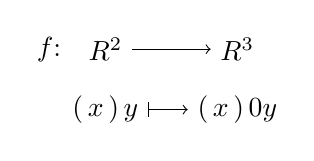
\begin{tikzpicture}[node distance=1mm]
        \node (functionName) at (0, 0) {$f$:};
        \node[right = of functionName] (domain) {$R^2$};
        \node[right = 1cm of domain] (codomain) {$R^3$};
        \node[below = 2mm of domain] (element) {$\begin{pmatrix}
                x \\
                y
            \end{pmatrix}$};
        \node at (element-|codomain) (image) {$\begin{pmatrix}
                x \\
                0 \\
                y
            \end{pmatrix}$};
        \draw[->] (domain) -- (codomain);
        \draw[|->] (element) -- (image);
    \end{tikzpicture}
\end{minipage}
\hfill
\begin{minipage}{0.35\linewidth}
    \begin{enumerate}[label=\protect\circled{\arabic*}]
        \item $f \in \mathcal{L}(R^2,R^3) ?$
        \item Kerf = ?
        \item Imf = ?
    \end{enumerate}
\end{minipage}
\begin{enumerate}[label=\protect\circled{\arabic*}]
    \item Necessary condition: $f(0_{E}) = 0_{F}$ : 
    $f(0_{R^2}) = \begin{pmatrix} 0 \\ 0 \end{pmatrix} 
    \rightarrow \begin{pmatrix} 0 \\ 0 \\ 0 \end{pmatrix}$ ?
    \[\forall (\alpha, X, Y) \in \mathbb{R} \times  \mathbb{R}^2 \times \mathbb{R}^2, X = \begin{pmatrix} x \\ y \end{pmatrix} \text{ and } Y = \begin{pmatrix} x' \\ y' \end{pmatrix}, x,y,x',y' \in \mathbb{R}\]
    \[f(\alpha \cdot X + Y) = \begin{pmatrix} \alpha \cdot x + x' \\ \alpha \cdot y + y' \end{pmatrix} = \begin{pmatrix} \alpha \cdot x + x' \\ 0 \\ \alpha \cdot y + y' \end{pmatrix} = \alpha \cdot \begin{pmatrix} x \\ 0 \\ y \end{pmatrix} + \begin{pmatrix} x' \\ 0 \\ y' \end{pmatrix} = \alpha \cdot f(X) + f(Y)\]
    so \circled{1} $f \in \mathcal{L}(R^2,R^3)$ \checkmark
    \item $Ker(f) = \left\{ \begin{pmatrix} x \\ y \end{pmatrix} \in R^2, \begin{pmatrix} x \\ 0 \\ y \end{pmatrix} = \begin{pmatrix} 0 \\ 0 \\ 0 \end{pmatrix} \right\} = \left\{ \begin{pmatrix} 0 \\ 0 \end{pmatrix} \right\}$
    \item $Im(f) = \left\{ \begin{pmatrix} x \\ 0 \\ y \end{pmatrix}, (x,y) \in R^2 \right\} = \left\{ x \begin{pmatrix} 1 \\ 0 \\ 0 \end{pmatrix} + y \begin{pmatrix} 0 \\ 0 \\ 1 \end{pmatrix}, (x,y) \in R^2 \right\}$ 
    \\$Im(f) = span\left\{ \begin{pmatrix} 1 \\ 0 \\ 0 \end{pmatrix}, \begin{pmatrix} 0 \\ 0 \\ 1 \end{pmatrix} \right\}$
\end{enumerate}
\subsection{Proposition}
\begin{enumerate}
    

    \item Let $f \in \mathcal{L}(E,F)$ and $g \in \mathcal{L}(F,G)$. Then: \[g \circ f \in \mathcal{L}(E,G)\]
    \item If $f$ is bijectif then $f{^{-1}}$ is bijective and $f{^{-1}} \in \mathcal{L}(F,E)$
    \item $\mathcal{L}(E,F)$ is a $\mathbb{K}-VS$:
        \newline
        \begin{minipage}{0.40\linewidth}
            
            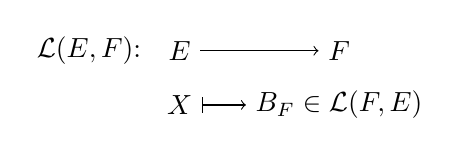
\begin{tikzpicture}[node distance=1mm]
                \node (functionName) at (0, 0) {$\mathcal{L}(E,F)$:};
                \node[right = of functionName] (domain) {$E$};
                \node[right = 1.5cm of domain] (codomain) {$F$};
                \node[below = 2mm of domain] (element) {$X$};
                \node at (element-|codomain) (image) {$B_F \in \mathcal{L}(F,E)$};
                \draw[->] (domain) -- (codomain);
                \draw[|->] (element) -- (image);
            \end{tikzpicture}
        \end{minipage}
        \hfill
        \begin{minipage}{0.59\linewidth}
            \begin{align*}
                \forall (\alpha, f, g) \in \mathbb{K} \times &\mathcal{L}^2(E,F) \\
                \alpha \cdot f + g \in &\mathcal{L}(E,F)
            \end{align*}
        \end{minipage}
\end{enumerate}
\end{document}